\newcommand{\cm}{\mathrm{cm^{-1}}}
\newcommand{\nm}{\mathrm{nm}}
\newcommand{\pltw}{0.8\textwidth}
\newcommand{\picwidth}{0.40\textwidth}
\newcommand{\unc}{0.3}  % uncertainty in nm
\section{Evaluation}

\subsection{Measuring bias of spectrometer}
To be able to identify the absorption spectrum of the iodine 2 molecule, we have to analise 
the measurements for callibration with the Na- and Hg-vapour lamps, respectively. The measured
spectrum over the entire range of the spectrometer is plotted in figure \ref{fig:specturm_all}. 
To locate the maxima, we magnify the recordings in a region around the corrispoding maximum. 
For sodium, this is done in figure \ref{fig:na_max}. One can see the two characteristic peaks 
at 
\begin{eqnarray*}
    \lambda_\mathrm{max, 1} = 589.1 \pm \unc \nm \\
    \lambda_\mathrm{max, 2} = 589.6 \pm \unc \nm.
\end{eqnarray*}
The uncertainty of \unc is taken from the value given in \cite{}, being half the value of 
resolution (6nm). It corrisponds with the sharpness of the maxima 
(fwhm about 0.4nm as seen in the figures). 
These corrispond with the values given in literature \cite{}, namely 
\begin{eqnarray*}
    \lambda_\mathrm{max, 1} = 589.0 \nm \\
    \lambda_\mathrm{max, 2} = 589.6 \nm.
\end{eqnarray*}
In the recorded spectrum, we also see another, smaller peak at 
\begin{equation}
    \lambda = 588.4 \pm \unc \nm.
\end{equation} 
This peak is not found in literature \cite{nist} and seems to be an artefact of the measurement. 
In fact, as the light from the Na lamp was not colliminated and focused very well, one could 
suspect diffration at the entrance of the spectrometer as the cause, as the spectrometer 
doesn't measure wavelength directly but rather the intensity corrisponding to a certain angle. 

For the Hg lamp, we observe similar results. As seen in \ref{fig:spectrum_all}, intensities 
of the minima varied quiet drastically. For that reason, we took various measurements of which 
we can use one for the first maximum (fig. \ref{fig:hg1_max}) and another at much lower 
intensity for the three other ones (figs. \ref{fig:hg2_max}, \ref{fig:hg3_max}). 
We identify the following maxima:
\begin{eqnarray*}
    \lambda_\mathrm{max, 1} &=& 435.5 \pm \unc \ (435.83)\nm \\
    \lambda_\mathrm{max, 2} &=& 545.9 \pm \unc \ (545.9)\nm \\
    \lambda_\mathrm{max, 3} &=& 576.8 \pm \unc \ (576.8)\nm \\
    \lambda_\mathrm{max, 4} &=& 576.9 \pm \unc \ (576.9)\nm.
\end{eqnarray*}
The values in parenthesis cite literature values \cite{}. \\
As the spectrometer yields results lying within the literature values for the 
stated uncertainty, we conclude that there is no bias in the measured wavelength.

\begin{figure}
\centering
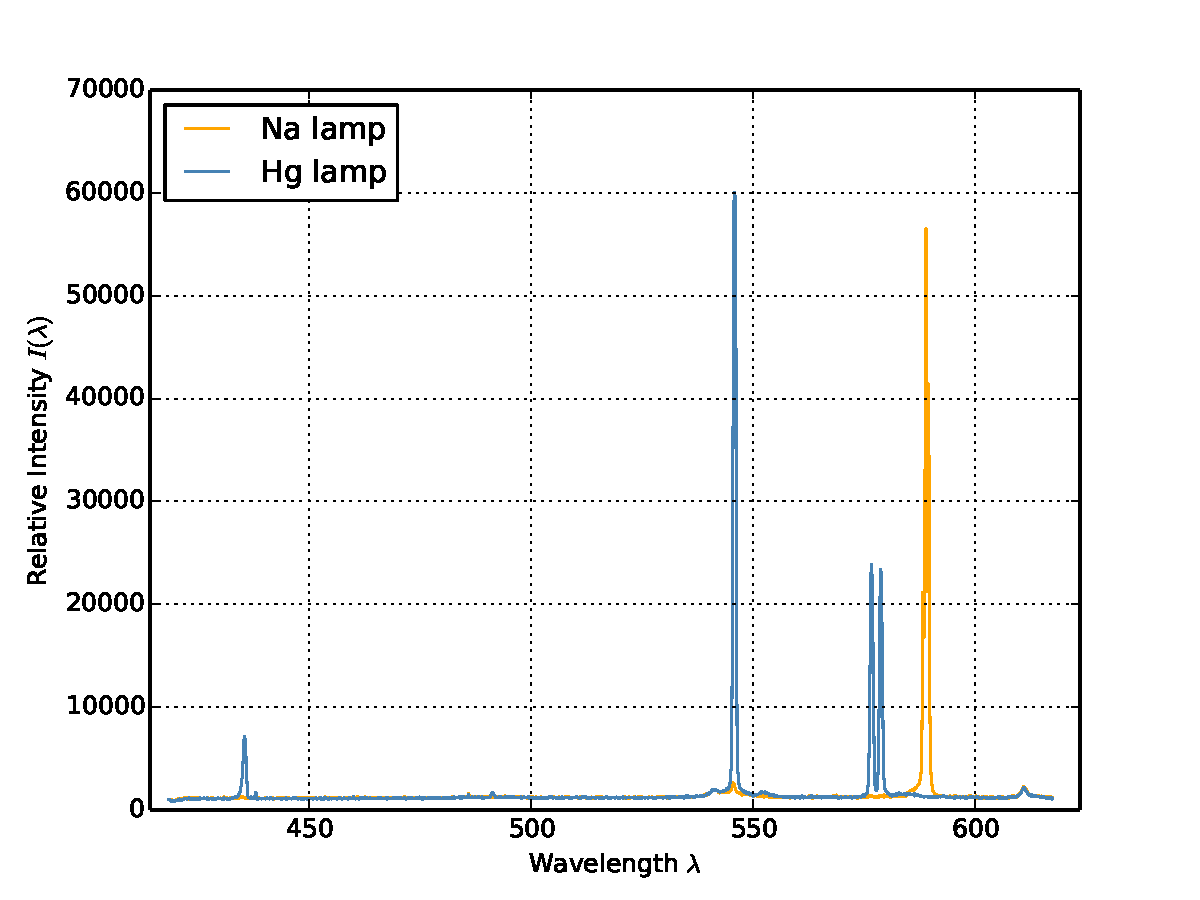
\includegraphics[width=\pltw]{analysis/figures/spectrum_all.pdf}
\caption{Measured spectrum of Na and Hg lamp}
\label{fig:spectrum_all}
\end{figure}

\begin{figure}
\centering
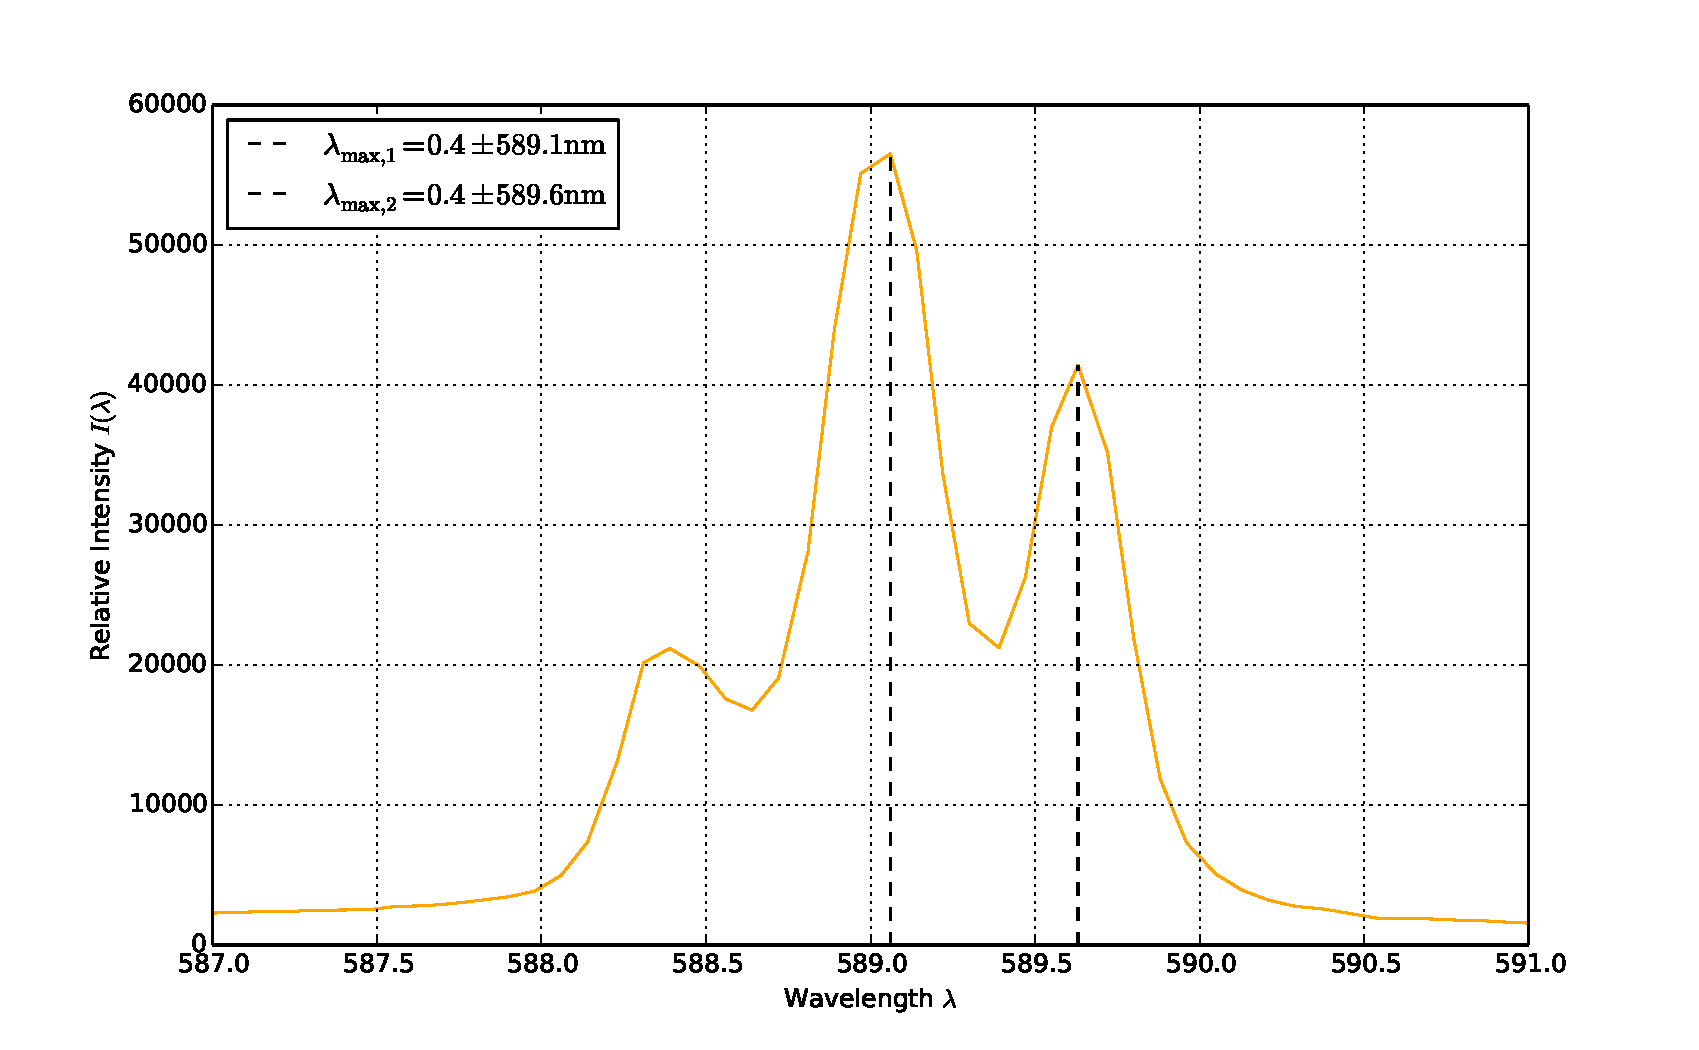
\includegraphics[width=\pltw]{analysis/figures/na_max.pdf}
\caption{Measured spectrum of the Na lamp, detail at the 
characteristic orange double line}
\label{fig:na_max}
\end{figure}

\begin{figure}
\centering
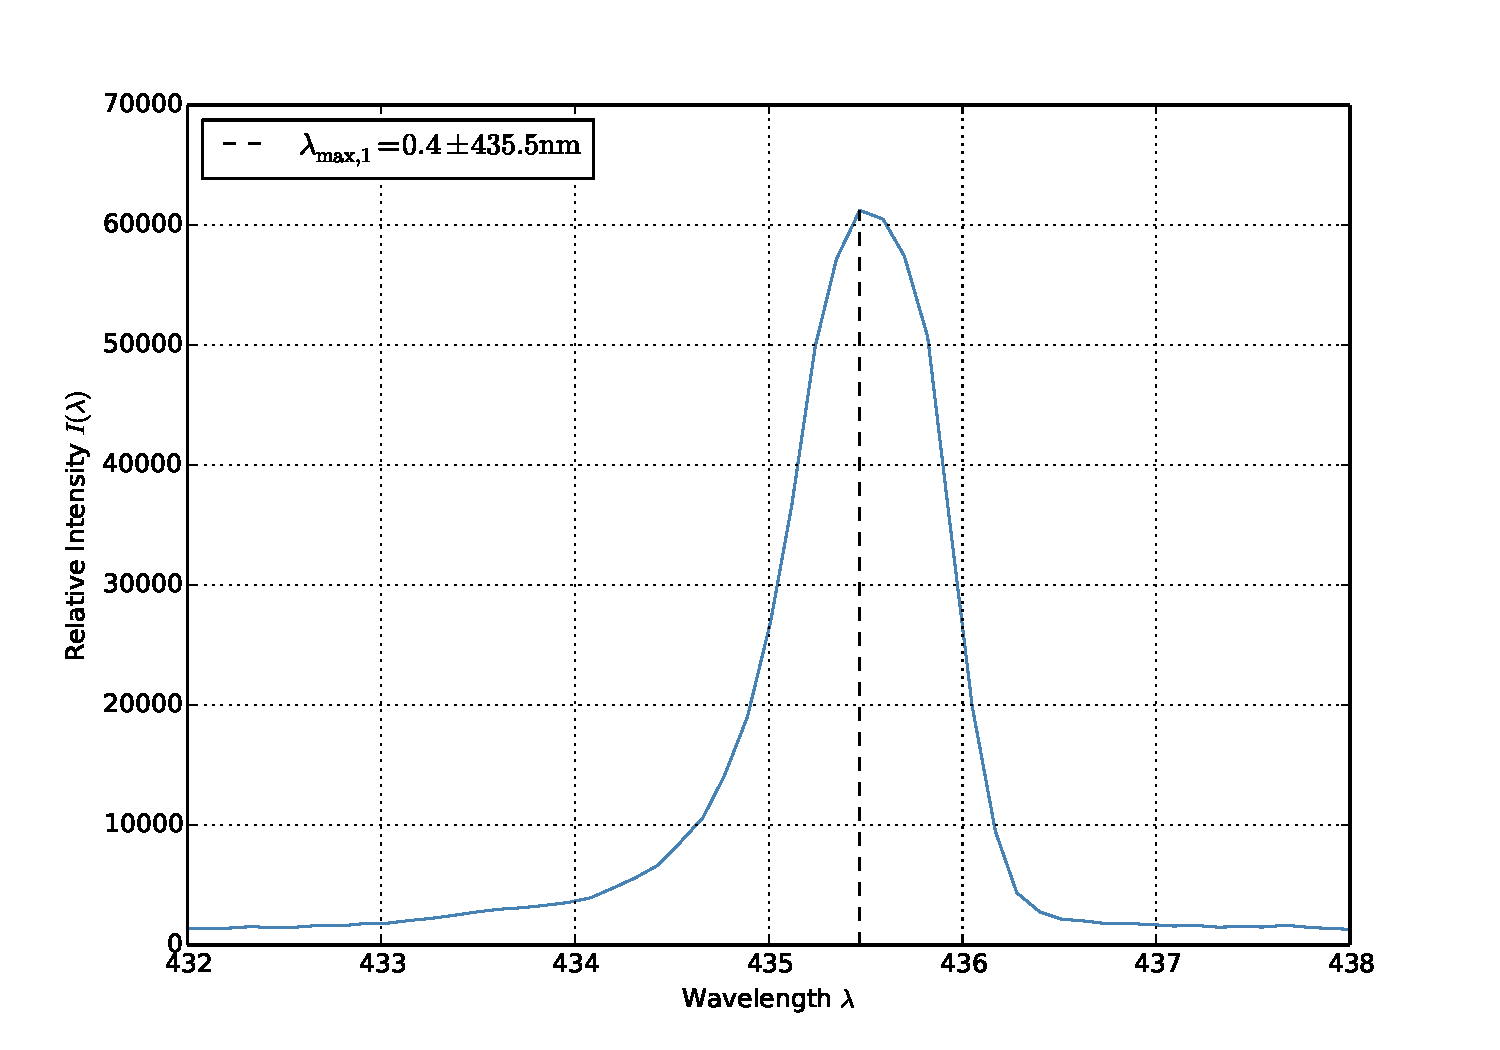
\includegraphics[width=\pltw]{analysis/figures/hg1_max.pdf}
\caption{Measured spectrum of the hg lamp, detail at first maximum}
\label{fig:hg1_max}
\end{figure}

\begin{figure}
\centering
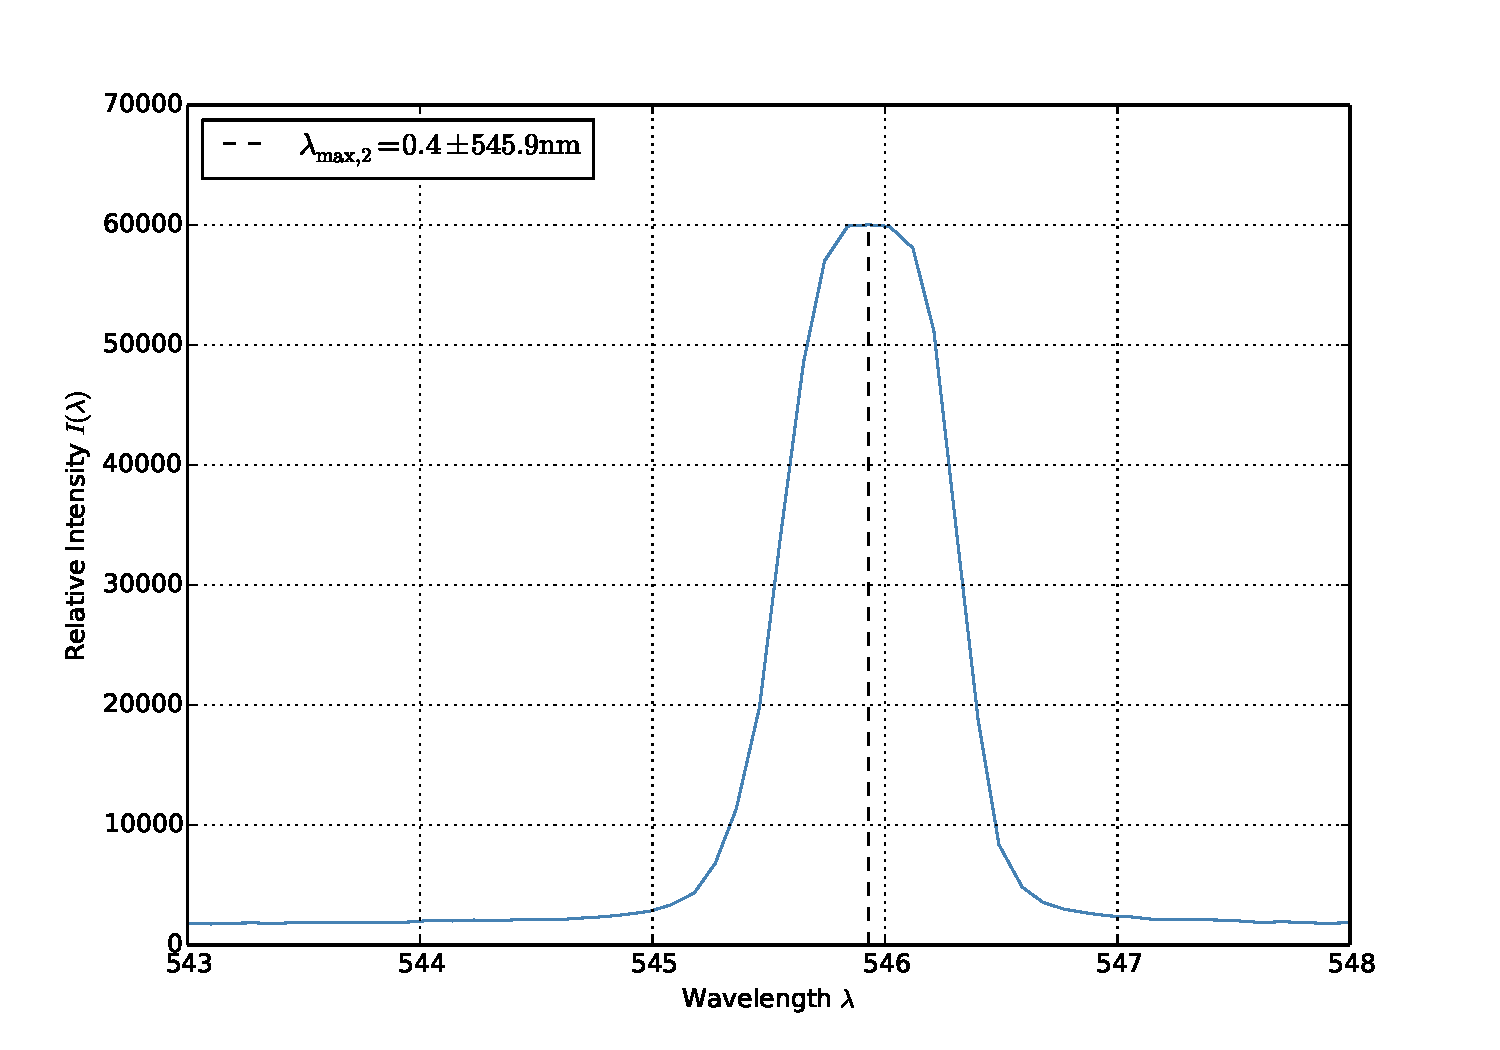
\includegraphics[width=\pltw]{analysis/figures/hg2_max.pdf}
\caption{Measured spectrum of the hg lamp, detail at second maximum}
\label{fig:hg2_max}
\end{figure}

\begin{figure}
\centering
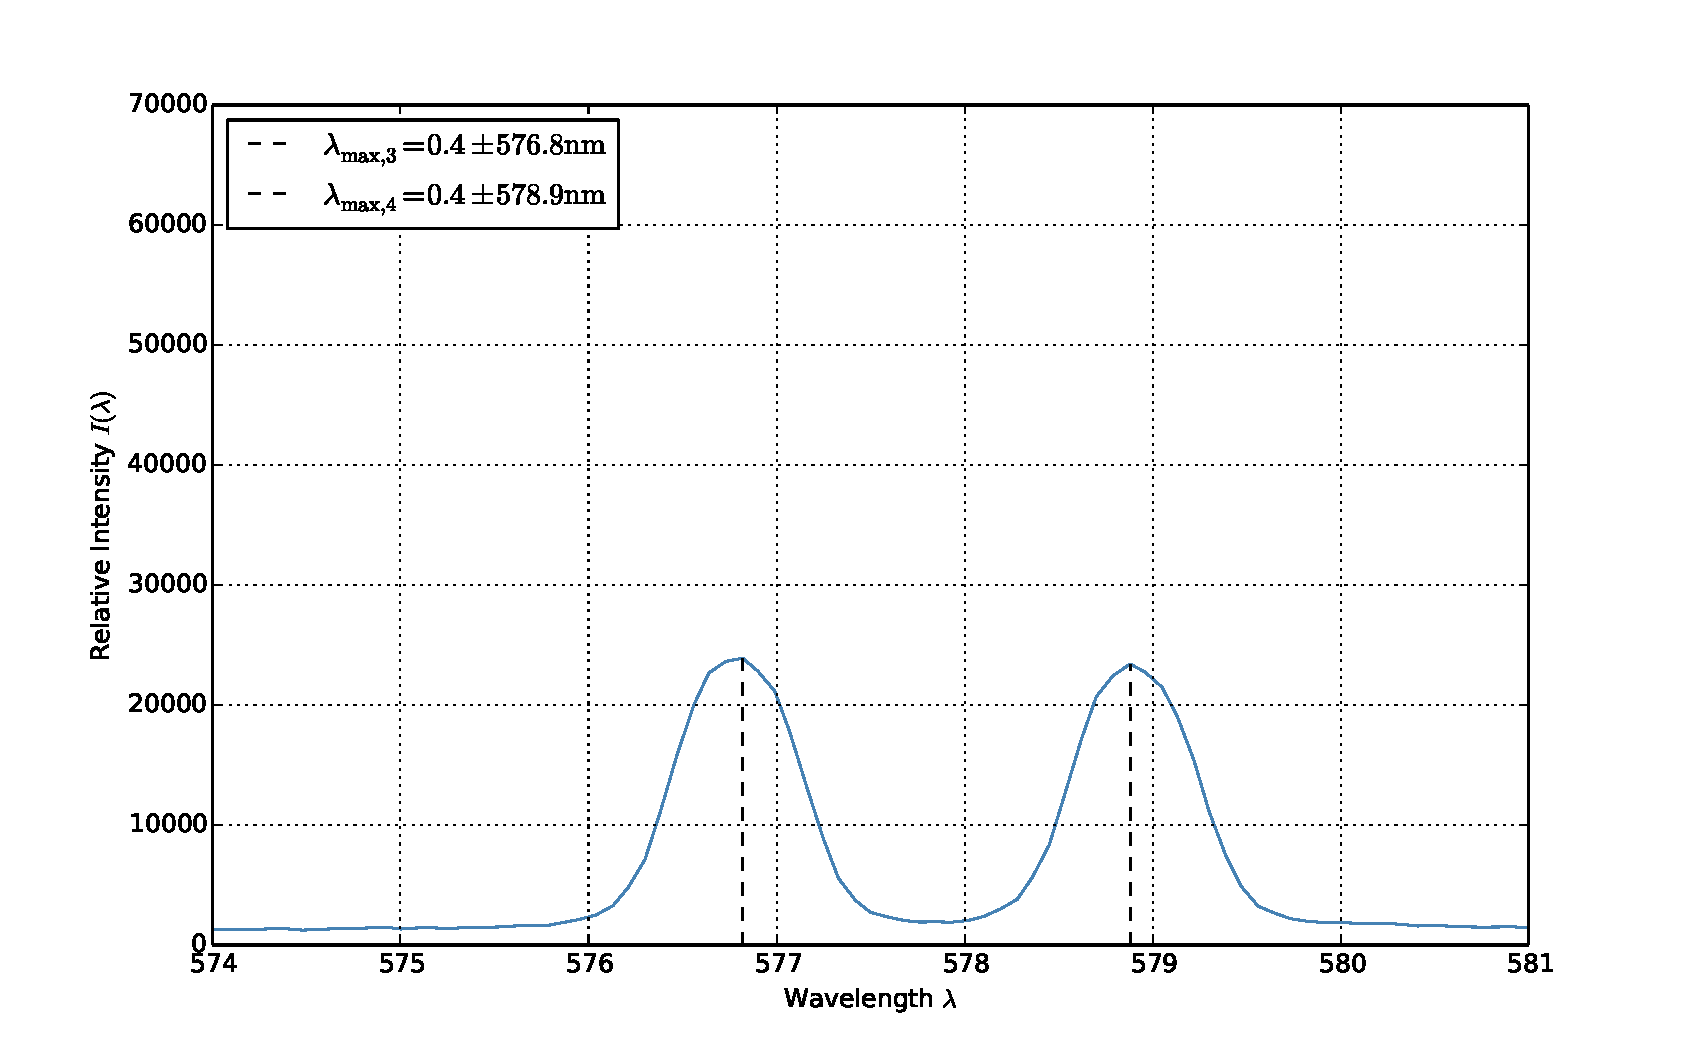
\includegraphics[width=\pltw]{analysis/figures/hg3_max.pdf}
\caption{Measured spectrum of the hg lamp, detail at thrid and fourth maximum}
\label{fig:hg3_max}
\end{figure}

\subsection{Spectrum of halogen lamp}
As we look out to measure the absorption spectrum of iodine, we first take a quick look at 
the specturm of the background from which photons are to be absorbed. The measured spectrum 
of the used halogen lamp within the range of wavelength in question is shown in figure 
\ref{fig:specturm_halogen_full}.
\begin{figure}
\centering
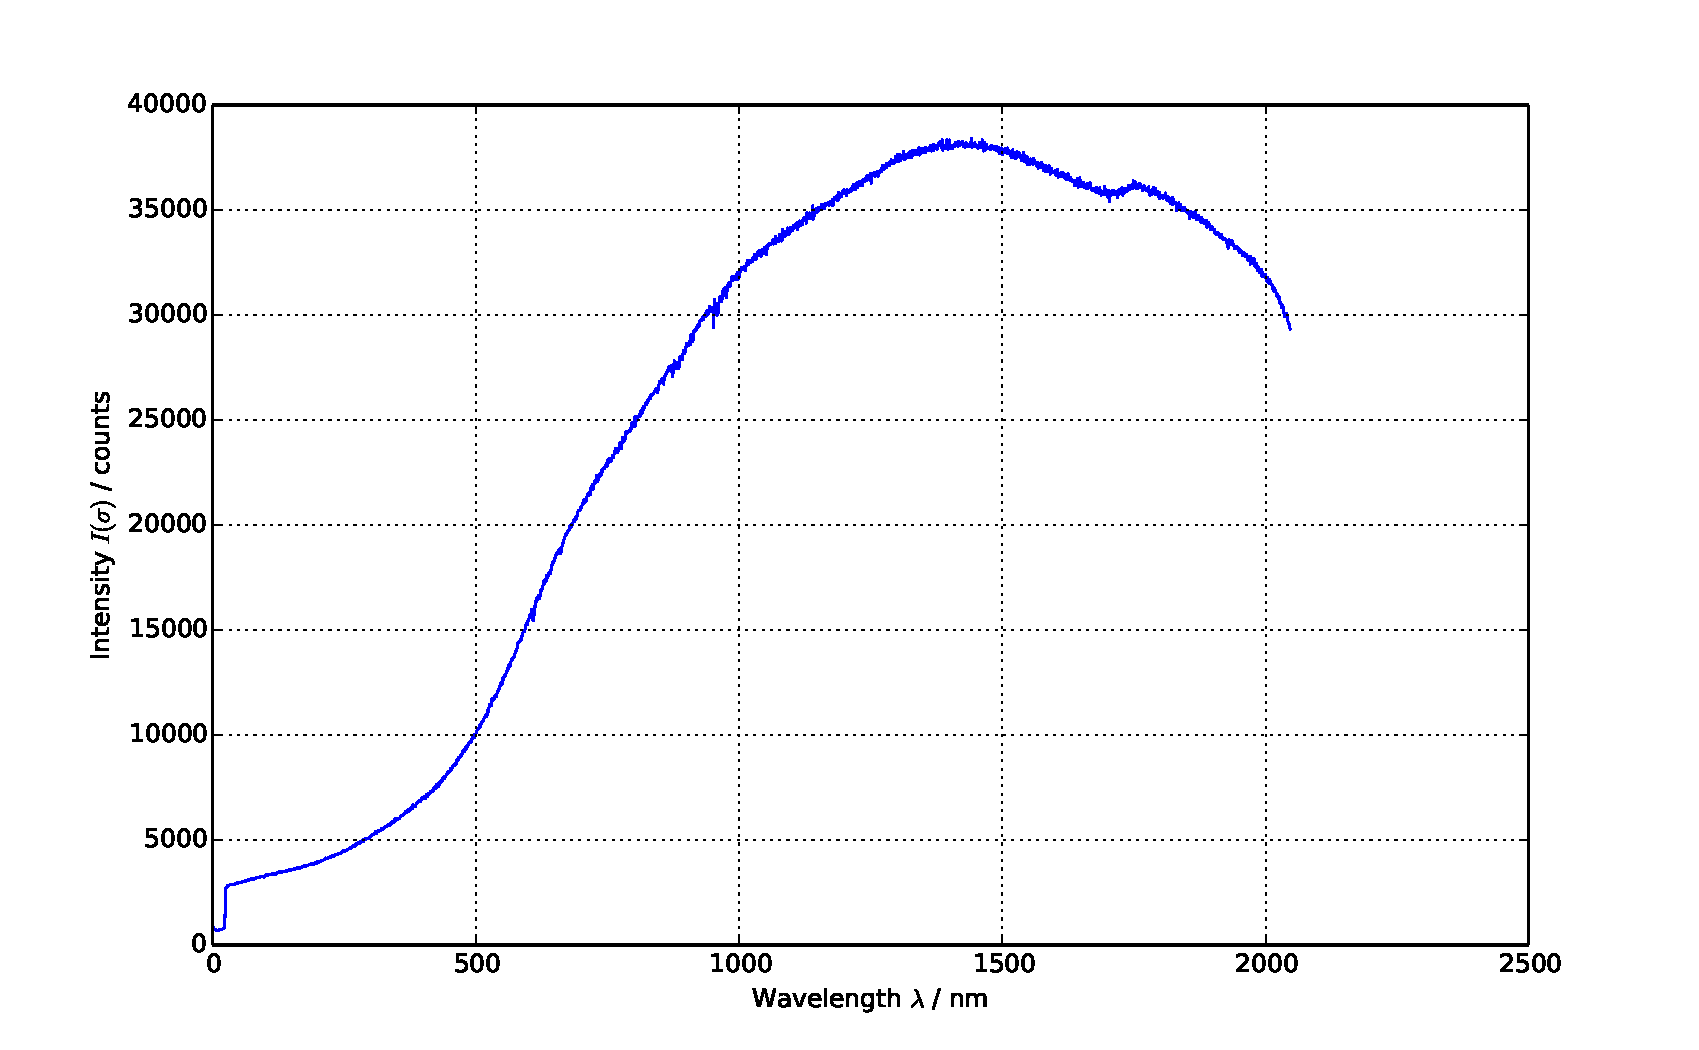
\includegraphics[width=\pltw]{analysis/figures/halogen_02.pdf}
\caption{Measured spectrum of the halogen lamp over the entire spectrum, no coerrection for 
diffraction in light}
\label{fig:spectrum_halogen_full}
\end{figure}
To be able to compare this to the absorption spectrum, we firth need to make the same 
corrections for diffraction in light as we do for the latter. We do so by linearly 
interpolating given literature values of the diffraction index, given in table 
\ref{tab:diff_air}.

\begin{table}[h]
\centering
\begin{tabular}{| c |l|l|l|l|}
\hline
$\lambda [\nm]$              & 680  & 600  & 540  & 500 \\ \hline
$(n_\mathrm{air} - 1) \cdot 10^{-4}$ & 2.76 & 2.77 & 2.78 & 279 \\ \hline
\end{tabular}
\caption{Diffraction indices for air at room temperatur and normal pressure for 
chosen wavelength $\lambda$, taken from \cite{}.}
\label{tab:diff_air}
\end{table}

The linear interpolation is done by the following equation:
\begin{eqnarray}
    n_\lambda &=& \frac{(2.79 - 0.01 j)}{10 ^{4}} - \
    \frac{(\lambda - \lambda_\mathrm{lower})} {10^{6} \cdot \
(\lambda_\mathrm{upper} - \lambda_\mathrm{lower})} + 1 \\
    \lambda &=& n_\lambda \, \lambda,
    \label{eqn:lin_interpol}
\end{eqnarray}
where j is the index of the collum of table \ref{tab:diff_air} within which $\lambda$ lies, 
$\lambda_\mathrm{upper}$ and $\lambda_\mathrm{lower}$ are the upper and lower bounds of the 
intervall (more precisely: $\lambda \in (\lambda_\mathrm{upper}, \lambda_\mathrm{lower}]$ ). 

The corrected values of $\lambda$ are now restricted to values of 
$\lambda \in [500\nm, 620\nm]$ and converted to $\cm$ by taking th inverse. The result 
can be observed in figure \ref{"fig:spectrum_halogen_red"}.
\begin{figure}
\centering
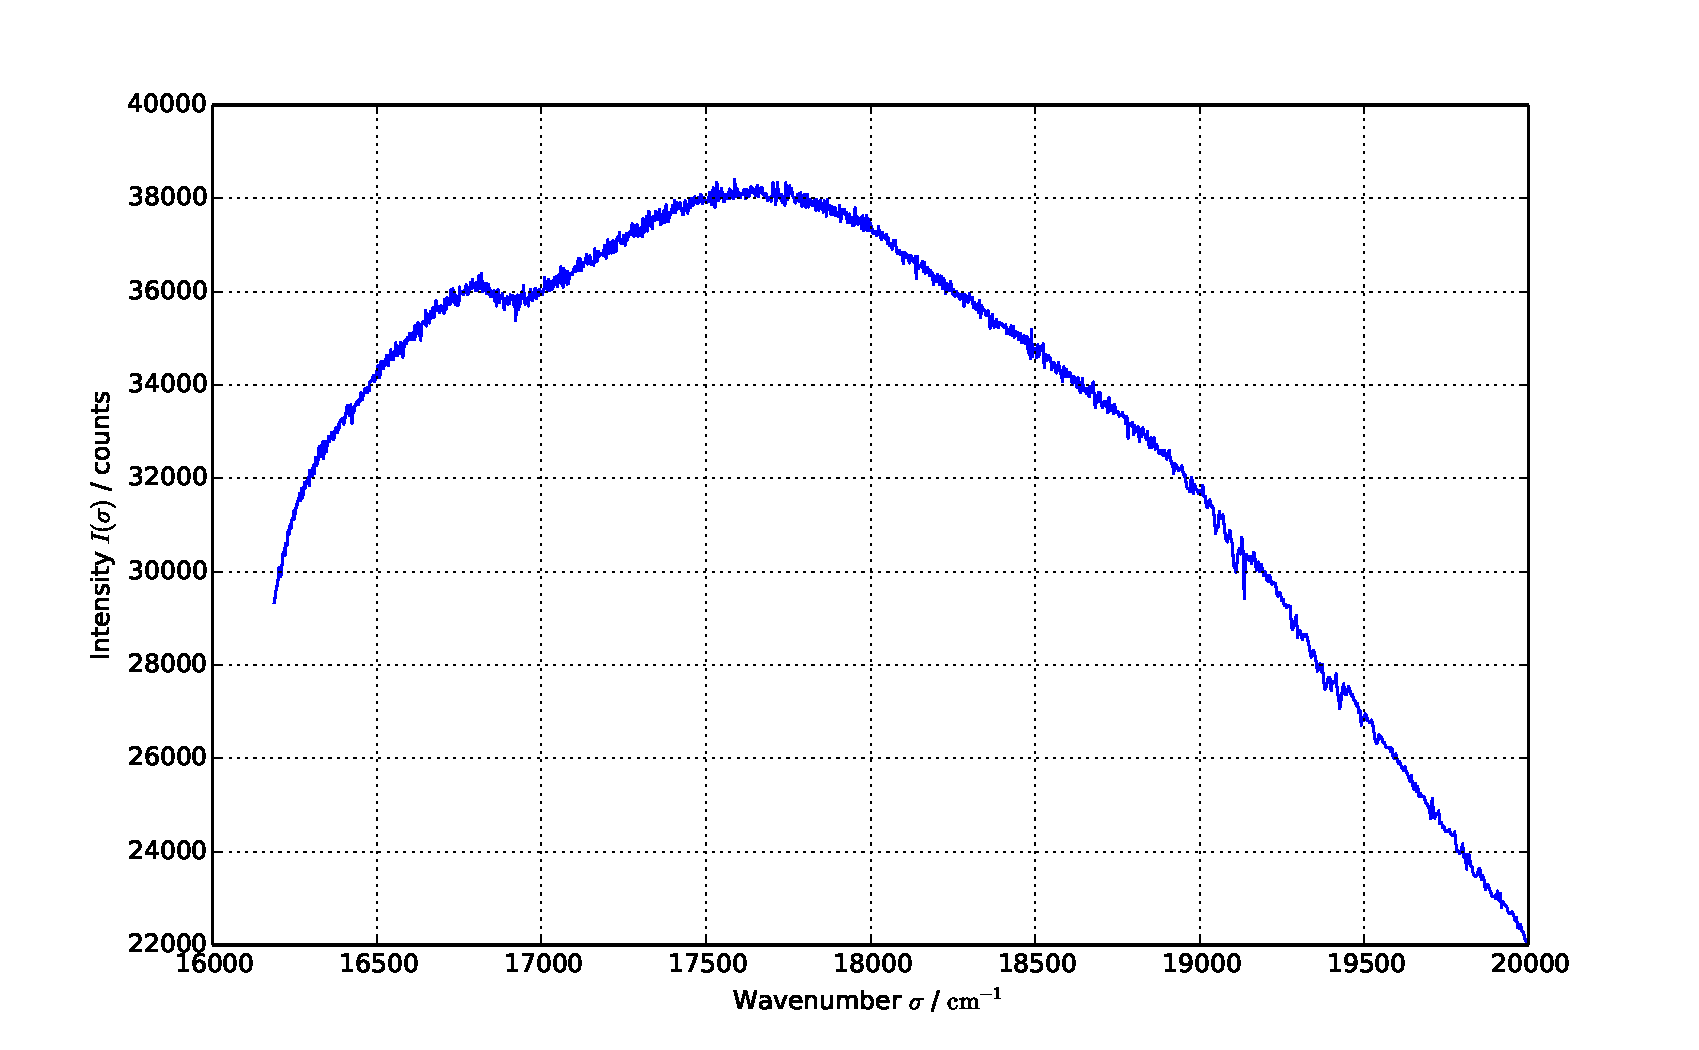
\includegraphics[width=\pltw]{analysis/figures/halogen_red.pdf}
\caption{Measured spectrum of the halogen lamp over the entire spectrum, no correction for 
diffraction in light}
\label{fig:spectrum_halogen_red}
\end{figure}


\subsection{Identifying progressions}
The process of identifying progressions turned out to be quiet difficult – reflecting the 
rather unsteady course of history. 
The absorption spectrum and the found progressions are shown in figure \ref{fig:absorp}.
The measured wavelenghts are reduced to vacuum wavelength by equation \eqref{eqn:lin_interpol} 
and then transformed to wavenumbers in $\cm$. 
As a first step, we preselected minima by an algorithm checking for each point to be lower than 
its four neighbouring points and added further points by hand later on. For identifying corrisponding 
progression to each of the selected points, we used the starting point of the 'zeroth progression' 
$v'' = 0  \rightarrow v' = 25$ with a band at $545.8 \nm = 18321 \cm$, as given by \cite{}. In our 
measurement, we found a mimima at $E_{0, 25} = 18319 \pm 10\nm$. From that line, we could first 
identify the progression members down to $v' = 47$, where the last three points could be added using 
the first order approximation of the energy differences, namely their negative linear correlation 
to the energy (see figure \ref{fig:absorp_detail_03}). We then used the same relationship to identify 
points for $v' < 25$, which overlap with point of the progression $v''(1) \rightarrow v'$, the 
'first progression', 
as shown in figure \ref{fig:absorp_detail_02}. For this progression, we found much less values, as 
it overlaps with the progression $v''(1) \rightarrow v'$, 'second progression', as well, as one can 
observe in figure \ref{fig:absorp_detail_01}. All identified points with respective wavenumbers 
$\sigma_{v'', v'}, v'' \in \{0, 1, 2\}$ are shown in table \ref{tab:prog}, 
while the energy differences $\Delta G_{v''}(v' + 1 / 2) = \sigma_{v'', v'} - \sigma{v'', v' + 1}$ are 
listed in table \ref{tab:prog}.

\begin{table}[h]
\centering
\footnotesize
\begin{tabular}{|l |l |l ||c|
                 l |l |l ||c|
                 l |l |l ||c|
                 l |l |l |}
\hline
$v'$ & $\frac{\sigma_{0,v'}}{\cm}$ & $\frac{\Delta \sigma_{0,v'}}{\cm}$ &&
$v'$ & $\frac{\sigma_{0,v'}}{\cm}$ & $\frac{\Delta \sigma_{0,v'}}{\cm}$ &&
$v'$ & $\frac{\sigma_{1,v'}}{\cm}$ & $\frac{\Delta \sigma_{1,v'}}{\cm}$ &&
$v'$ & $\frac{\sigma_{2,v'}}{\cm}$ & $\frac{\Delta \sigma_{2,v'}}{\cm}$ \\ \hline
47 & 19587 & 11 & &32 & 18830 & 10 & &27 & 18262 & 10 & &20 & 17468 & 9 \\ \hline
46 & 19549 & 11 & &31 & 18761 & 10 & &26 & 18184 & 9 & &19 & 17375 & 9 \\ \hline
45 & 19513 & 11 & &30 & 18693 & 10 & &25 & 18105 & 9 & &18 & 17282 & 8 \\ \hline
44 & 19475 & 11 & &29 & 18623 & 10 & &24 & 18021 & 9 & &17 & 17186 & 8 \\ \hline
43 & 19433 & 11 & &28 & 18547 & 10 & &23 & 17938 & 9 & &16 & 17090 & 8 \\ \hline
42 & 19383 & 11 & &27 & 18472 & 10 & &22 & 17856 & 9 & &15 & 16990 & 8 \\ \hline
41 & 19338 & 11 & &26 & 18398 & 10 & &21 & 17765 & 9 & &14 & 16888 & 8 \\ \hline
40 & 19289 & 11 & &25 & 18318 & 10 & &20 & 17678 & 9 & &13 & 16782 & 8 \\ \hline
39 & 19241 & 11 & &24 & 18237 & 9 & &19 & 17589 & 9 & &12 & 16675 & 8 \\ \hline
38 & 19186 & 11 & &23 & 18153 & 9 & &18 & 17495 & 9 & &11 & 16570 & 8 \\ \hline
37 & 19135 & 10 & &22 & 18066 & 9 & &17 & 17399 & 9 & &10 & 16463 & 8 \\ \hline
36 & 19077 & 10 & &21 & 17979 & 9 & &16 & 17300 & 8 \\ \cline{1-11}
35 & 19020 & 10 & &20 & 17891 & 9 \\ \cline{1-7}
34 & 18956 & 10 & &19 & 17802 & 9 \\ \cline{1-7}
33 & 18896 & 10 & &18 & 17706 & 9 \\ \cline{1-7}
\end{tabular}
\caption{Identified members of progressions of vibrational modes $v'' \rightarrow v'$ 
and corrisponding wavenumbers $\sigma_{v'', v'} = G'(v') - G''(v'').$}
\label{tab:prog}
\end{table}

\begin{table}[h]
\centering
\footnotesize
\begin{tabular}{|l |l |l ||c|
                 l |l |l ||c|
                 l |l |l ||c|
                 l |l |l |}
\hline
$v' + \frac{1}{2}$ & $\frac{\Delta G_{0} }{ \cm} $ & $\frac{\Delta (\Delta G) }{ \cm} $&&
$v' + \frac{1}{2}$ & $\frac{\Delta G_{0} }{ \cm} $ & $\frac{\Delta (\Delta G) }{ \cm} $&&
$v' + \frac{1}{2}$ & $\frac{\Delta G_{1} }{ \cm} $ & $\frac{\Delta (\Delta G) }{ \cm} $&&
$v' + \frac{1}{2}$ & $\frac{\Delta G_{2} }{ \cm} $ & $\frac{\Delta (\Delta G) }{ \cm} $\\ \hline
46 & 38 & 16 & & 31 & 68 & 14 & & 26 & 77 & 14 & & 19 & 92 & 12 \\ \hline
45 & 35 & 16 & & 30 & 68 & 14 & & 25 & 79 & 13 & & 18 & 93 & 12 \\ \hline
44 & 38 & 16 & & 29 & 70 & 14 & & 24 & 84 & 13 & & 17 & 96 & 12 \\ \hline
43 & 42 & 16 & & 28 & 76 & 14 & & 23 & 82 & 13 & & 16 & 96 & 12 \\ \hline
42 & 49 & 15 & & 27 & 75 & 14 & & 22 & 81 & 13 & & 15 & 99 & 12 \\ \hline
41 & 44 & 15 & & 26 & 74 & 14 & & 21 & 91 & 13 & & 14 & 101 & 12 \\ \hline
40 & 48 & 15 & & 25 & 79 & 14 & & 20 & 87 & 13 & & 13 & 106 & 12 \\ \hline
39 & 48 & 15 & & 24 & 81 & 14 & & 19 & 88 & 13 & & 12 & 107 & 11 \\ \hline
38 & 55 & 15 & & 23 & 83 & 14 & & 18 & 94 & 13 & & 11 & 104 & 11 \\ \hline
37 & 51 & 15 & & 22 & 87 & 13 & & 17 & 95 & 12 & & 10 & 106 & 11 \\ \hline
36 & 57 & 15 & & 21 & 86 & 13 & & 16 & 98 & 12 & & 9 & 107 & 11 \\ \hline
36 & 57 & 15 & & 20 & 88 & 13 & & 15 & 104 & 12 \\ \cline{1-11}
34 & 64 & 15 & & 19 & 89 & 13 \\ \cline{1-7}
33 & 59 & 15 & & 18 & 96 & 13 \\ \cline{1-7}
32 & 66 & 15 \\ \cline{1-3}
\end{tabular}
\caption{Identified members of progressions of vibrational modes $v'' \rightarrow v'$ 
and corrisponding wavenumbers $\sigma_{v'', v'} = G'(v') - G''(v'').$}
\label{tab:dG}
\end{table}

\begin{figure}
    \centering
    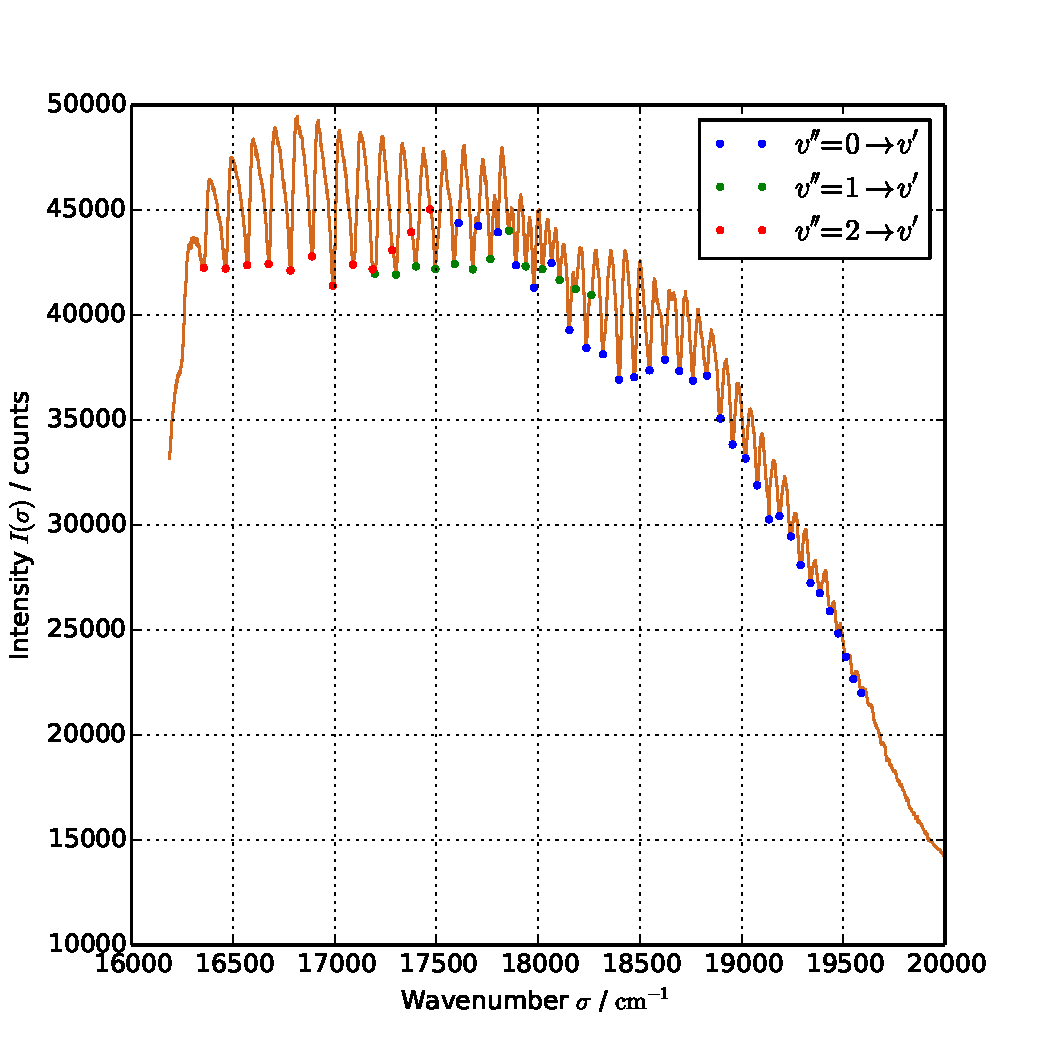
\includegraphics[width=\pltw]{analysis/figures/absorp_03.pdf}
    \caption{Measured spectrum of halogen lamp having passed the iodine pipe. The local minima are 
    those of the absorption spectrum of iodine. Three progressions of vibrational states $v'' \rightarrow v'$
    within the electronic transition 
    $B ^3\Pi_{\sigma \, \mathrm{u}}^{+} \quad \leftarrow \quad X ^1\Sigma_{\sigma \, \mathrm{u}}^{+}$ 
    are identified with colored dots. }
    \label{fig:absorp}
\end{figure}

\begin{figure}
    \centering
    \begin{subfigure}[b]{\picwidth}
        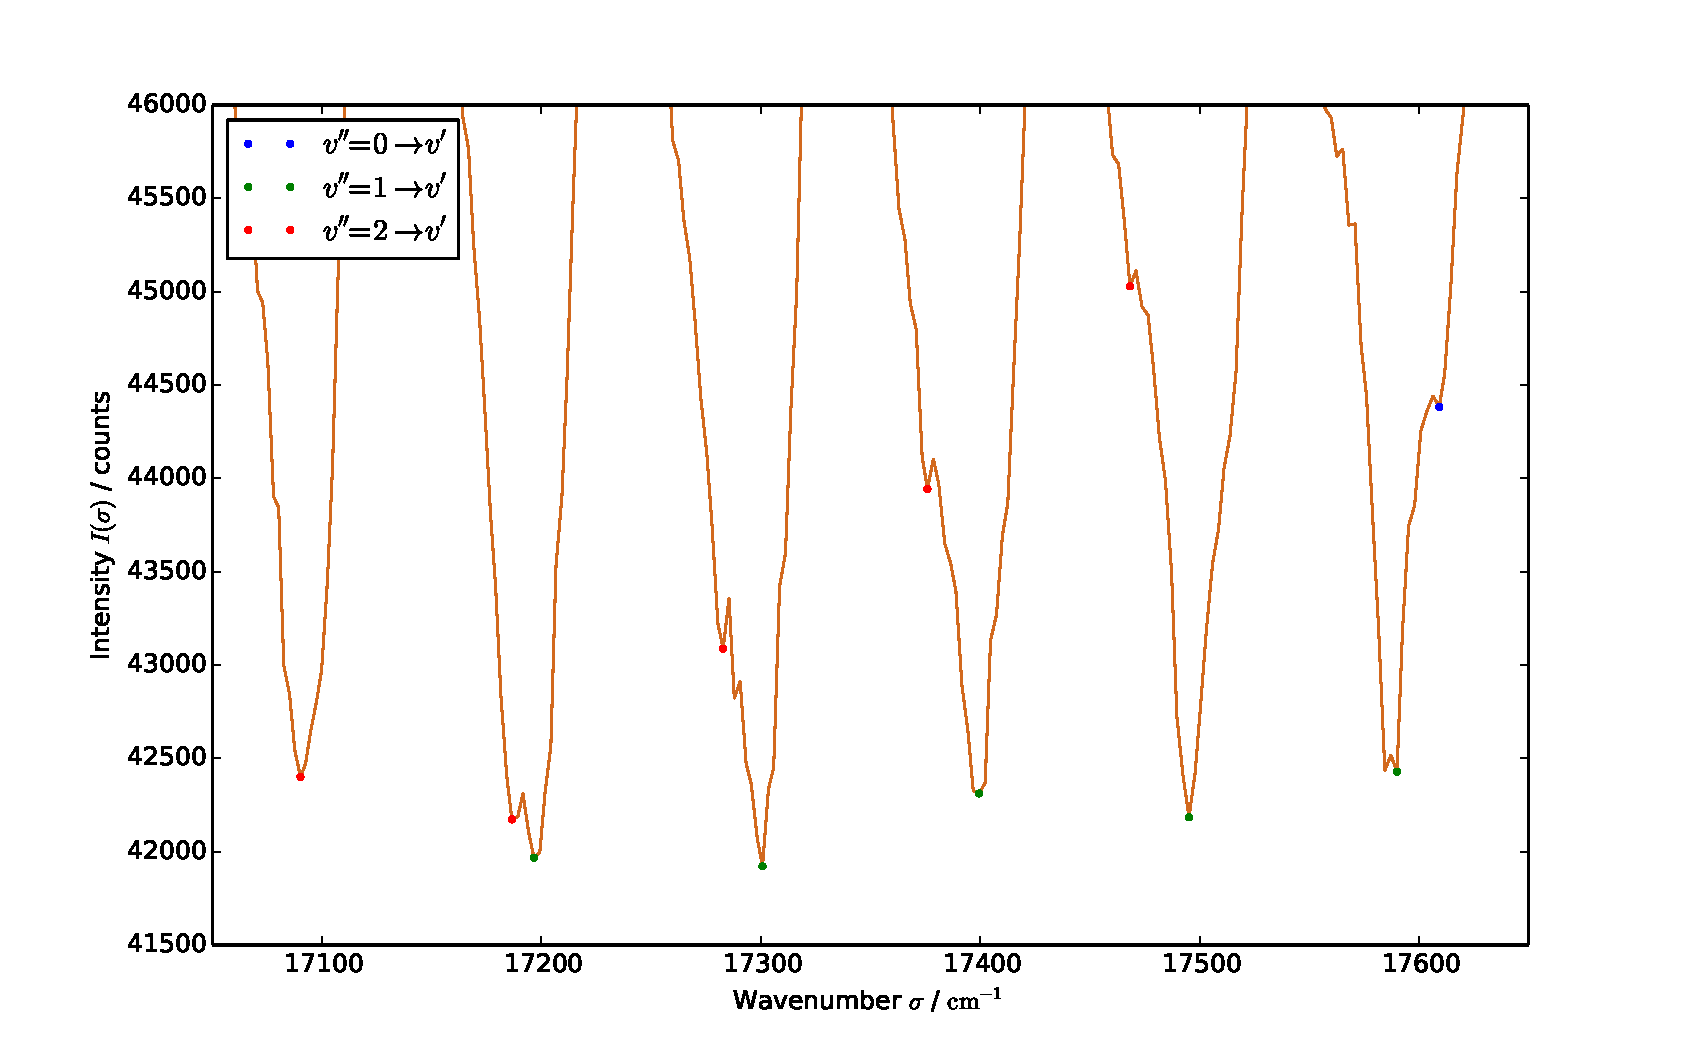
\includegraphics[width=\pltw]{analysis/figures/absorp_03_detail_01.pdf}
        \caption{Overlap of $v'=1$ and $v'=2$}
        \label{fig:absorp_detail_01}
    \end{subfigure}\qquad
    \begin{subfigure}[b]{\picwidth}
        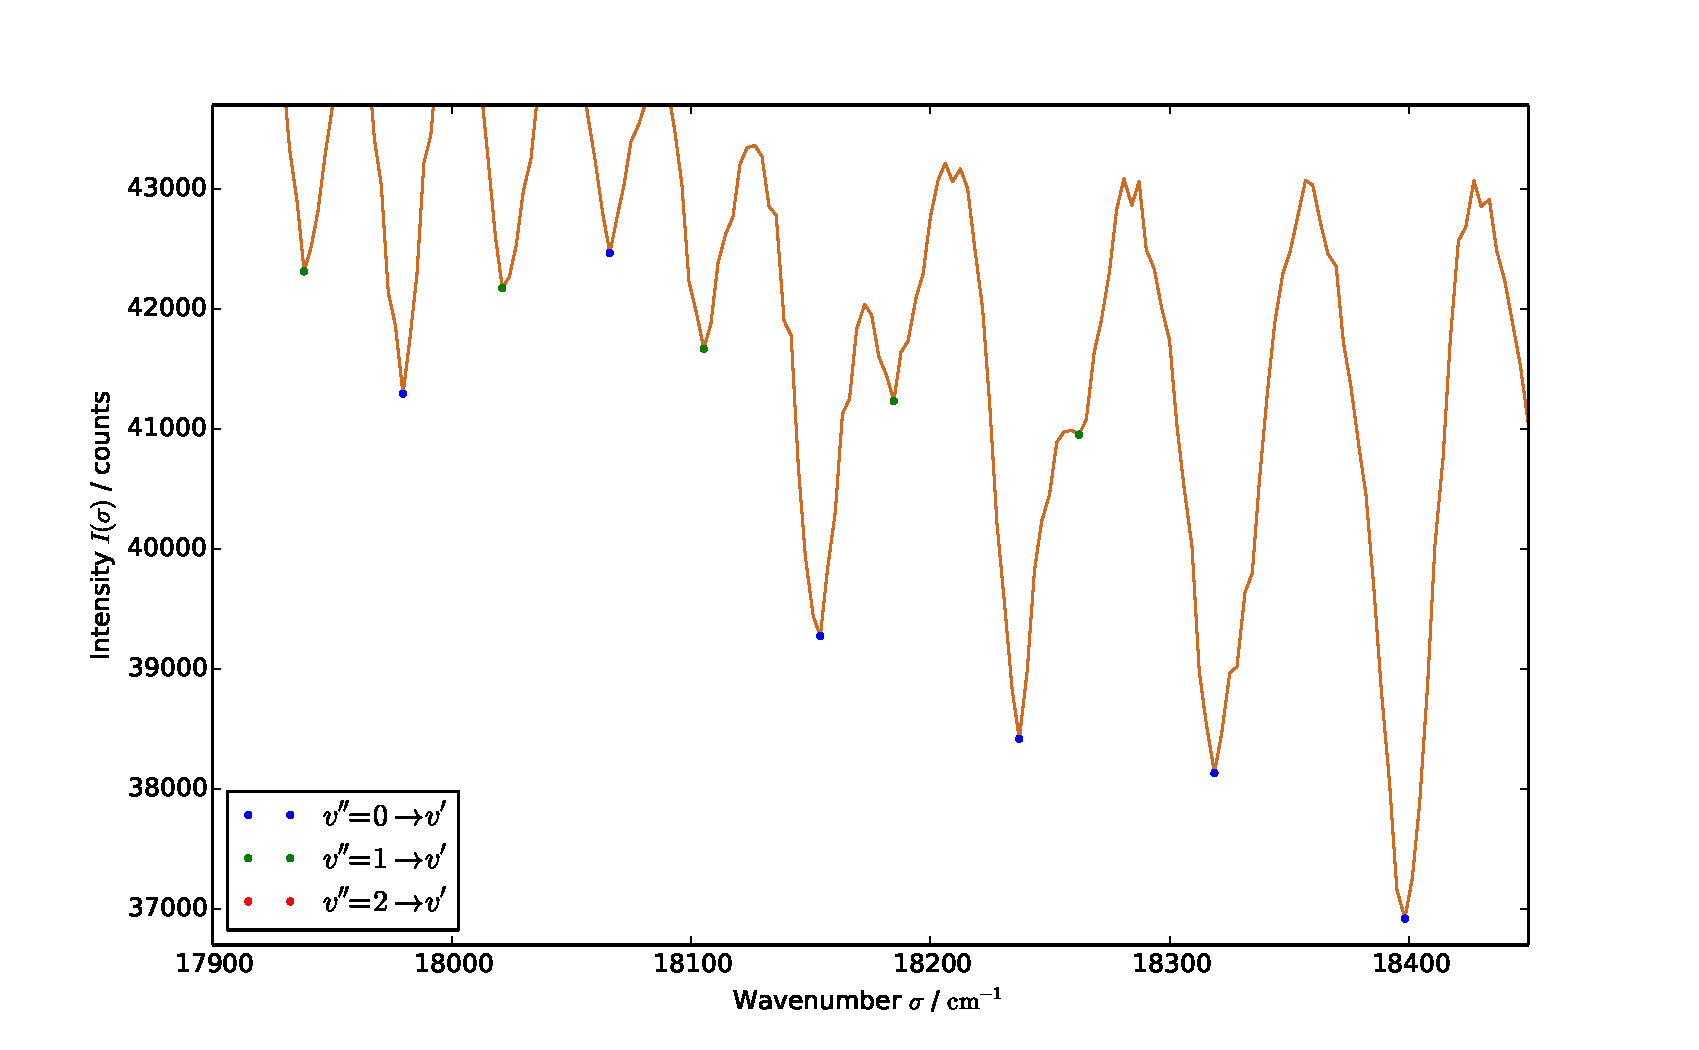
\includegraphics[width=\pltw]{analysis/figures/absorp_03_detail_02.pdf}
        \caption{Overlap of $v'=0$ and $v'=1$"}
        \label{fig:absorp_detail_02}
    \end{subfigure}
    \begin{subfigure}[b]{\picwidth}
        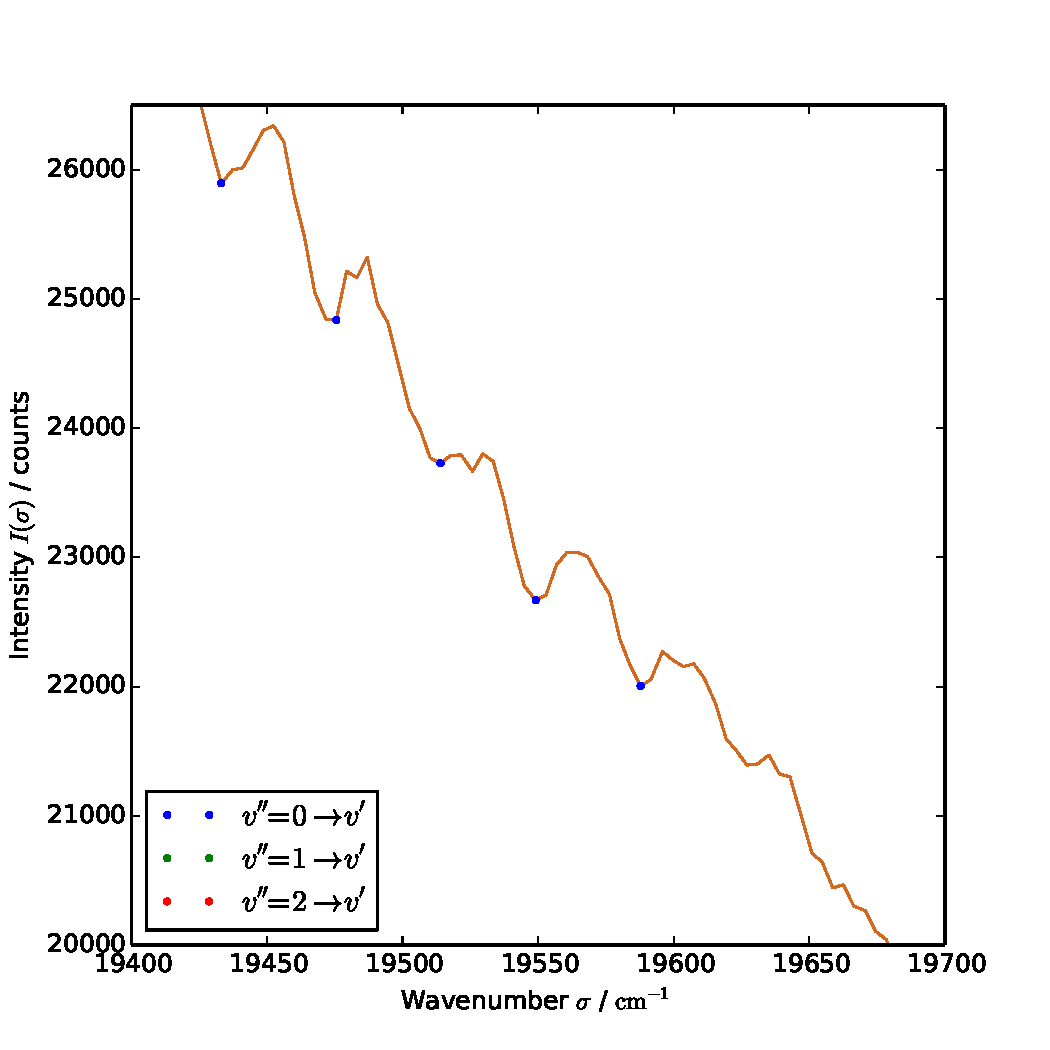
\includegraphics[width=\pltw]{analysis/figures/absorp_03_detail_03.pdf}
        \caption{End of $v'=0'$}
        \label{fig:absorp_detail_03}
    \end{subfigure}
    \caption{Details of \ref{fig:absorp}: members of progressions at points, where identification is not trivial, 
    but done by looking at the progression of energy differences.} 
    \label{fig:absorp_detail}
\end{figure}

The energy differences of the identified progressions are shown in the so-called Birge-Sponer plots, figures 
\ref{fig:b_s_0}, \ref{fig:b_s_1}, \ref{fig:b_s_2}
